\documentclass{article}
\usepackage{pgfplots}
\pgfplotsset{compat=1.18}
\usepgfplotslibrary{groupplots,fillbetween}
\usepackage{amsmath}
\begin{document}
\section{Functions}
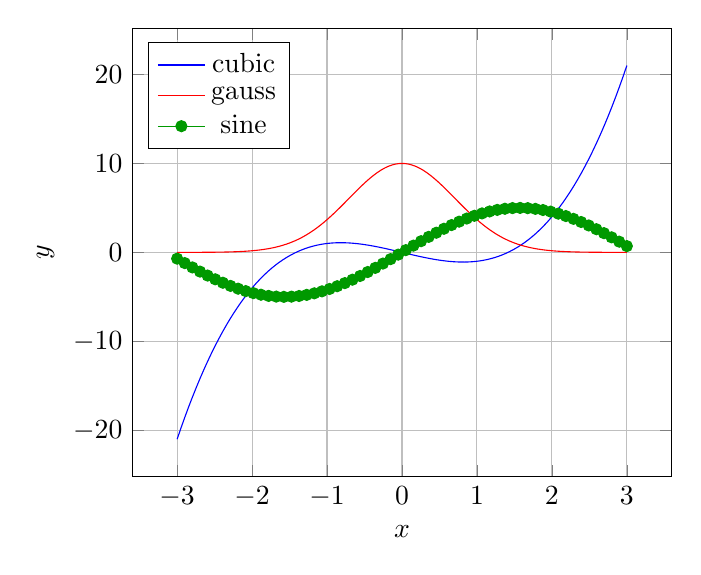
\begin{tikzpicture}
  \begin{axis}[xlabel=$x$, ylabel=$y$, legend pos=north west, grid=major]
    \addplot[blue, domain=-3:3, samples=120] {x^3 - 2*x};
    \addplot[red, domain=-3:3, samples=120] {exp(-x^2)*10};
    \addplot[green!60!black, domain=-3:3, samples=60, mark=*] {sin(deg(x))*5};
    \legend{cubic, gauss, sine}
  \end{axis}
\end{tikzpicture}
\section{Data}
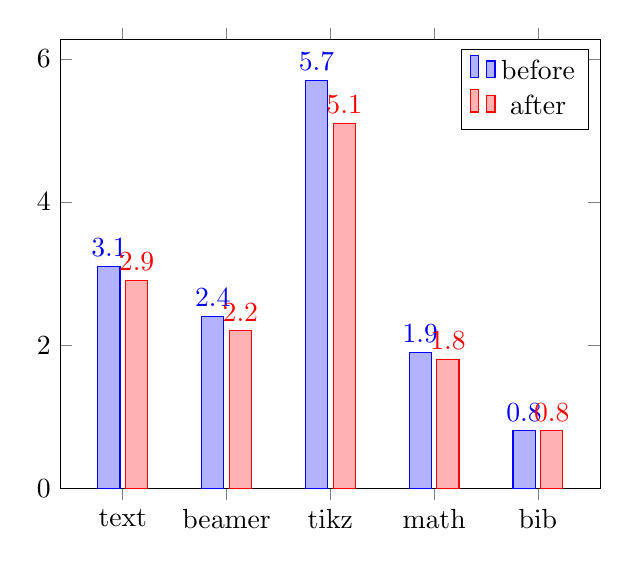
\begin{tikzpicture}
  \begin{axis}[ybar, symbolic x coords={text,beamer,tikz,math,bib}, xtick=data,
      nodes near coords, ymin=0, bar width=8pt, enlarge x limits=0.15]
    \addplot coordinates {(text,3.1) (beamer,2.4) (tikz,5.7) (math,1.9) (bib,0.8)};
    \addplot coordinates {(text,2.9) (beamer,2.2) (tikz,5.1) (math,1.8) (bib,0.8)};
    \legend{before, after}
  \end{axis}
\end{tikzpicture}
\begin{tikzpicture}
  \begin{loglogaxis}[xlabel={pages}, ylabel={ms}]
    \addplot table {
      x y
      1 12
      2 21
      4 40
      8 77
      16 160
      32 330
      64 640
      128 1300
    };
  \end{loglogaxis}
\end{tikzpicture}
\section{Groups}
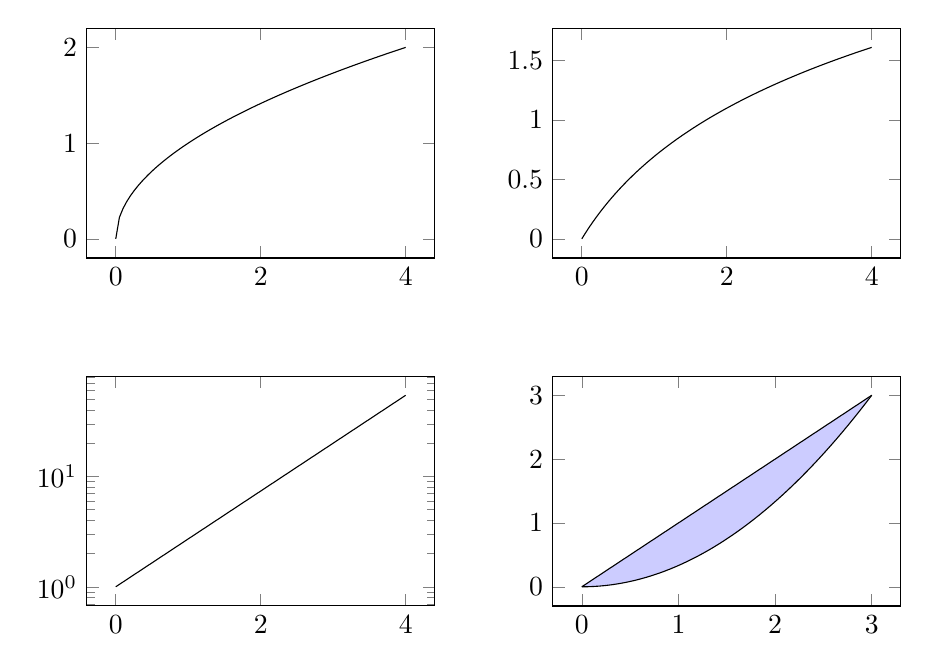
\begin{tikzpicture}
  \begin{groupplot}[group style={group size=2 by 2, horizontal sep=1.5cm, vertical sep=1.5cm},
      width=6cm, height=4.5cm]
    \nextgroupplot \addplot[domain=0:4, samples=80] {sqrt(x)};
    \nextgroupplot \addplot[domain=0:4, samples=80] {ln(x+1)};
    \nextgroupplot[ymode=log] \addplot[domain=0:4, samples=40] {exp(x)};
    \nextgroupplot
      \addplot[name path=f, domain=0:3, samples=50] {x^2/3};
      \addplot[name path=g, domain=0:3, samples=50] {x};
      \addplot[blue!20] fill between[of=f and g];
  \end{groupplot}
\end{tikzpicture}
\section{Surface}
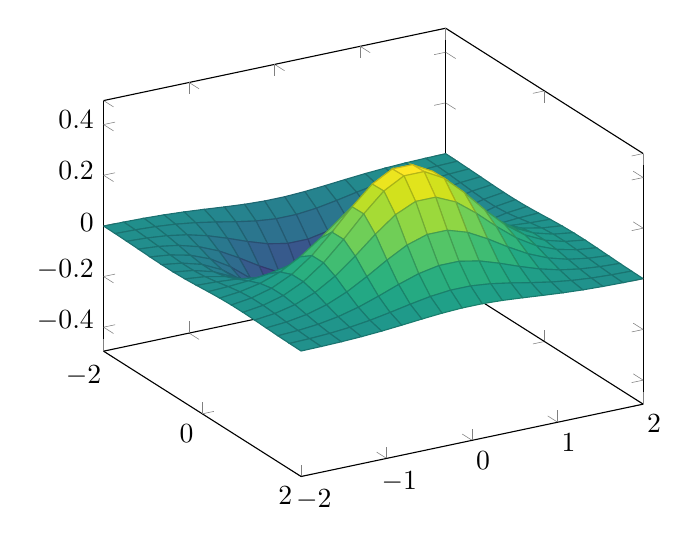
\begin{tikzpicture}
  \begin{axis}[view={60}{30}, colormap/viridis]
    \addplot3[surf, domain=-2:2, samples=18] {exp(-x^2-y^2)*x};
  \end{axis}
\end{tikzpicture}
\end{document}
